\chapter*{\Huge Synthesis and general discussion}
\thispagestyle{thesis} % Force the thesis page style
\markboth{\MakeMarkcase{Synthesis and general discussion}}{\MakeMarkcase{Synthesis and general discussion}} % Set headers
\addcontentsline{toc}{chapter}{Synthesis and general discussion} % Add to Table of Contents

\renewcommand{\thefigure}{SD.\arabic{figure}}
\setcounter{figure}{0}
\renewcommand{\thetable}{SD.\arabic{table}}
\setcounter{table}{0}

% 1. Implications of water-saving strategies (intro par, not section)

The concept of holistic management has been present in ecosystem research since the early 70's, stemming from the realization that biotic and abiotic system components are deeply interconnected \citep{risser1985toward}. Rice paddies follow this same principle and, as human-made wetlands, their management must account for potential effects on multiple roles inherent to such ecosystems \citep{fasola1996}. Due to their large contribution to GHG emissions, developing and assessing climate change mitigation practices are main objectives for most of the rice management research community \citep{zhang2023}. Such assessments have, nevertheless, been found to focus mainly on climate change and production issues \citep{vuciterna2024}, overlooking other important system dimensions. Water-saving irrigation strategies, proven efficient  practices decreasing CH$_{4}$ emissions \citep{jiang2019}, alter the hydrology of these systems and trigger effects on several biogeochemichal and ecological processes related to these water layers and saturated soils \citep{gharsallah2023}. % find more references
Therefore, these practices should be assessed considering their potential implications in the system as a whole.\\

Given the current global change context and the need to develop strategies that help limiting global warming while securing food supply to the growing population (i.e., SDGs 2 and 13, of zero hunger and urgent climate change action, respectively; \cite{unitednations2015}), the positive climate change mitigation represented by these strategies has driven large interest \citep{linquist2018, gao2024effects}.  Unfortunately, this interest often masks their potential negative effects. Throughout this work we have identified ecosystem trade-offs and system dimensions so far neglected across water-saving irrigation assessments. This might result particularly harmful for agroecosystems like the Ebro Delta, where natural and rice human-made wetlands are entangled through large extensions, hence representing important biodiversity hotspots \citep{ibanez2010}. In \textbf{Chapter \ref{Chapter1}}, trade offs with biodiversity conservation of different groups of aquatic organisms were described. Abundance and diversity declines for different groups of organisms when implementing water-saving strategies in rice fields have already been identified in different rice production areas \citep{watanabe2013, golet2018, herring2021}. We found the strategy intensity gradient as main driver of these negative effects, being stronger in AWD and milder in MSD, considered as severe and medium intensity practices, respectively. Therefore, MSD was considered as a more sustainable practice, alternative to AWD, as it maintained the positive climate change mitigation potential while not having such strong negative effects on biodiversity conservation. This was also achieved without grain yield declines compared to continuous flooding, as was the case for AWD.\\ 

Besides impacts on biodiversity, across \textbf{Chapter \ref{Chapter2}} the importance and often lack of consideration of the temporal dimension while assessing rice climate change mitigation practices were also described. Most scientific studies on water-saving strategies assessment have been conducted solely considering rice growing seasons \citep{linquist2015, kumar2019alternate}. While flooded fallow season CH$_{4}$ emissions, and the effects these strategies may have on them, have been found non-significant in some temperate lowland rice production areas \citep{lahue2016}, that is not always the case. As previously described by \cite{martinez-eixarch2018}, fallow CH$_{4}$ emissions represented the highest contribution (87 \%) to overall annual emissions within our system. Furthermore, the widely described positive AWD effect decreasing emissions during growing seasons \citep{carrijo2017} was inverted during the fallow period. We described how legacy effects of water-saving practices implemented during the growing season on the structure of soil microbial communities might drive a decrease in AWD climate change mitigation potential during fallow seasons. Progressive adaptation of microbial communities in paddy soils to irrigation practices define emission patterns in longer time scales \citep{lagomarsino2016}, highlighting the importance of considering temporal dimensions in water-saving strategies assessments.\\

Finally, \textbf{Chapter 3} widened the assessment scope considering an agroecosystem multifunctionality approach. Besides CH$_{4}$ emissions (i.e., an agroecosystem disservice) and biodiversity conservation (i.e., an agroecosystem service), rice paddies are involved in the provision of multiple other ecosystem services \citep{chivenge2020}. Water \citep{ye2013, lampayan2015}  and nitrogen \citep{cheng2022} use efficiency, soil organic carbon storage \citep{livsey2019}, and food provision \citep{carrijo2017}, had already been pointed out as services susceptible to non-continuous flooding regimes. Very few studies have centered their focus in identifying trade-offs driven by the implementation of water-saving strategies \citep{gao2024effects, vitali2024}. Although no overall multifunctionality effects were identified in our study for any of the assessed practices, these had effects on individual services and assessment indicators. While some abundance and diversity indicators were positively affected by water-saving practices when compared to continuous flooding (e.g., higher coleoptera diversity under both MSD and AWD), other groups of organisms suffered strong abundance declines (e.g., fish and amphibians in AWD plots). Other indicators affected by irrigation practices were soil particulated organic carbon, predation rate of chironomid larvae, and crayfish abundance. Grain yield was significantly reduced under AWD irrigation. High heterogeneity outcomes among indicators lead to no significant links between agroecosystems.\\

\begin{figure*}[htbp]
\centering
\vspace{0pt}
\begin{minipage}[t]{0.35\textwidth}
\vspace{0pt} % Forces top alignment inside minipage
\captionsetup{width=\linewidth, justification=justified}
\captionof{figure}[Landscape implementation of water-saving strategies]{Implementation of water-saving practices in rice paddies considering both temporal and landscape scales tacling ecological trade-offs between climate change mitigation and biodiversity conservation objectives. Adapted from \citep{perez-mendez2025a} (\textit{unpublished manuscript}), illustration: Scienseed.}
\label{Landscp}
\end{minipage}%
\hfill
\begin{minipage}[t]{0.6\textwidth}
\vspace{0pt}
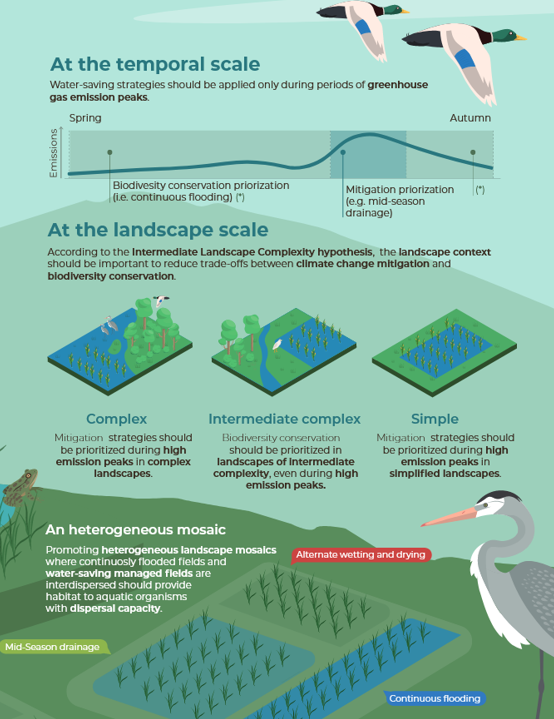
\includegraphics[scale=0.7]{Figures/ldscp_water.png}
\end{minipage}
\end{figure*}

Considering ecological trade-offs between climate change mitigation and biodiversity conservation, the effects on temporal emission dynamics and changes in agroecosystem multifunctionality in the assessment of water-saving strategies contributes to the closing of knowledge gaps in rice ecosystem management. The realization that no particular irrigation practice is overall positive for the whole ecosystem, as they all entail mitigation-biodiversity, temporal and multifunctional trade-offs, is consistent throughout this Thesis. As in previous studies with wider assessment scopes \citep{watanabe2013}, % look for more
our holistic assessment leads us to recommend a heterogeneous mosaic of irrigation practices rather than favoring single strategies. Under a mosaic approach, continuously flooded paddies would aim for biodiversity conservation objectives serving as refuge for species able to disperse in between fields, while fields managed under non-continuous flooding would help mitigating overall landscape CH$_{4}$ emissions. Water-saving strategies implemented on large scales, without continuously flooded patches, can drive towards absolute depletion of some susceptible groups of organisms (e.g., amphibians under AWD; \textbf{Chapter \ref{Chapter1}}). This management heterogeneity would also secure that no particular agroecosystem service (i.e., biodiversity conservation, supporting-regulating and provision services) is affected negatively on large extensions. For instance, extensive negative impacts on soil particulated organic carbon might be observed under paddy landscapes managed solely under water-saving irrigation strategies. Similarly, rice ecosystems managed uniquely under AWD might result in important grain yield losses.\\ 

As discussed by \cite{perez-mendez2025a} (\textit{unpublished manuscript}), assessing the implementation of water-saving irrigation practices should respond to a spatiotemporal perspective (Figure \ref{Landscp}). At a temporal scale, both growing seasons should be considered. During the growing season, water-saving practices should be applied according to emission records obtained from continuously flooded fields, targeting CH$_{4}$ emission peaks, while maintaining continuous flooding during the rest of the season.  Maximum emission mitigation occurs when field drains are applied at \citep{fertitta-roberts2019}, or right before \citep{souza2021}, expected peaks. As described in \textbf{Chapter \ref{Chapter1}}, timely implementation of intermediate intensity (i.e., within a water use gradient) water-saving strategies, such as MSD, achieve decreasing CH$_{4}$ emissions while buffering strong negative biodiversity impacts of more intense strategies (i.e., AWD). Hence, this temporal approach when designing water management plans in rice paddies balances climate change mitigation and biodiversity conservation goals. Regarding fallow seasons, further research is needed to determine the best water management approach to tackle CH$_{4}$ emissions, as water-saving outcomes during growing seasons might result inverted after harvests (\textbf{Chapter \ref{Chapter2}}). Such effects respond to legacy effects of past water management in rice paddies on soil organic matter and microbial community structures, driving changes in GHG production and emission rates \citep{shao2017, tian2022}.  %cite maite studies on post harvest
At a landscape scale, \cite{perez-mendez2025a} propose planning rice water management based on the field spatial context, according to the intermediate landscape complexity hypothesis. In the context of rice paddies, this hypothesis sets landscapes of intermediate complexity (i.e., those where rice fields are dominant but have some remaining seminatural habitats) as those most susceptible to negative effects on biodiversity conservation and the provision of agroecosystem services under the implementation of water-saving strategies \citep{tscharntke2005landscape, bommarco2013ecological, grab2018}. Water-saving strategies should, therefore, be avoided in such landscapes, prioritizing biodiversity conservation objectives. Conversely, continuous flooding with timely MSD implementations would be a sustainable approach on simple and complex fields, as potential negative biodiversity effects would be buffered in the first case by nearby freshwater habitats, and in the second by communities consisting solely of high dispersing species (due to their distance to any other habitat sources).\\

Our proposed assessment aims for the adoption of a more holistic scope, though we acknowledge that integrating product life cycle and wider ecosystem service perspectives from current assessment frameworks is necessary to achieve a more complete methodology that accounts for effects in all system dimensions. Life Cycle Assessment (LCA) and Ecosystem Services Assessment (ESA) are frameworks established to identify management effects on ecosystems through wide assessment perspectives, though both lacking further integration to achieve holistic evaluations \citep{delucapena2022}. Even though LCA, which focuses on a product's life-cycle (i.e., from raw material acquisition, through production processes and practices, until its disposal; \cite{finnveden2009}), has been considered a holistic approach \citep{urbaniec2017}, it lacks consideration on potential effects on ecosystem services \citep{zhang2010accounting, d2020review}. Regarding rice water management, for instance, LCA studies have assessed water saving strategies mostly from a GHG emissions perspective, leading to conclude AWD as an overall positive practice \citep{abdulrahman2019, leon2022}. A wider LCA assessment scope by \cite{darzi-naftchali2025}, who considered a series of indicators as proxies for effects on biodiversity and ecosystem health, identified mostly positive global warming and water use efficiency outcomes related to AWD, overseeing potential trade-offs with other agroecosystem services. An assessment framework that tackles this, by considering ecosystem services as the basis for studying trade-offs between land use scenarios under different management practices, is that of ESA \citep{baskent2020}. This method has also been considered as a holistic assessment framework, although the lack of consensus on ecosystem service identification and valuation for proper assessments is still its greatest challenge \citep{menzie2012}. Rice water-saving management assessments using ESA methodology have identified several agroecosystem services within paddies, but focus as well mostly on GHG emissions, describing only related trade-offs (e.g., N$_{2}$O in relation to CH$_{4}$ emissions; \cite{chivenge2020}).\\

Holistic assessment of ecosystem management practices transcends rice paddy irrigation strategies, as these principles stand for any given systems. Our proposed spatiotemporal implementation of water-saving strategies in rice paddies stems from an evaluation process replicable across different ecosystems and management objectives. The described framework is consistent with \cite{vanderwilde2021}, who, through a bibliometric review on ecosystem services and LCA, identifies the use of Geographic Information System (GIS) modeling tools focusing on land use as a promising approach to overcome current low interaction in between LCA and ESA assessments. Such models are designed to assess ecosystem services on different time and spatial scales, quantifying the effects different land use intensities and management practices can have on the provision of multiple ecosystem services (e.g., Integrated Valuation of Ecosystem Services and Tradeoffs - InVEST; \cite{stanford2011}). Further research into the integration of potential ecosystem trade-offs, temporal dimensions and implications on system multifunctionality within assessment models would provide tools that help avoiding the promotion of practices that might result unsustainable at large time and spatial scales. Along with multiple cases where practices have been encouraged lacking proper consideration of potential trade-offs within forest and agricultural systems \citep{veldman2015, felton2016, hof2018, cohen2021}, AWD is often described as a climate-smart practice, included within CSA frameworks, and its implementation promoted across heterogeneous rice production areas \citep{krishna2016climate, tivet2017climate, bwire2024, das2024}. This highlights the importance of developing holistic assessment frameworks that provide decision-makers with the necessary tools to avoid the implementation of practices that might result conflicting with ecosystem management goals. Only through such rational ecosystem planning, breaking from traditional carbon tunnel vision and widening assessment perspectives, can ecological trade-offs be avoided in the development of mitigation and adaptation practices that properly tackle global change challenges.\\ 

% elaborate on how these tools apply for different systems
% talk about current mitigation frameworks (e.g., CSA, NBS) and their trade-offs (case studies). bwire2024: AWD as CSA
% SDGs
% What's new about my study: lack of ES or MF assessments in water-saving strategies. Cite Vitali (some AWD trade-offs), Chivenge (only N2O-CH4 trade-off)
% Recommend holistic assessment method. Must include our deficiencies (i.e., considering MF demand-stakeholders; other LCA considerations: water-use, energy, ferilizers, pesticides...; ... )


% Restore normal figure and table numbering
\renewcommand{\thefigure}{\thechapter.\arabic{figure}}
\setcounter{figure}{0}

\renewcommand{\thetable}{\thechapter.\arabic{table}}
\setcounter{table}{0}
